\documentclass{beamer} 
\usepackage{dcolumn}
\usepackage{listings}
\lstset{basicstyle=\scriptsize, showspaces=false, showtabs=false, showstringspaces=false, breaklines, prebreak=..., tabsize=2}
\usepackage{graphicx}
\usepackage{textcomp}
\usepackage{url}
\usepackage{hanging}
\urlstyle{rm}
\newcolumntype{.}{D{.}{.}{-1}}
\newcolumntype{d}[1]{D{.}{.}{#1}}
\usetheme{JuanLesPins}
\setbeamertemplate{footnote}{%
  \hangpara{2em}{1}%
  \makebox[2em][l]{\insertfootnotemark}\footnotesize\insertfootnotetext\par%
}
\beamertemplatenavigationsymbolsempty


\title[]{Getting Started}
\subtitle{Introduction to Java}
\author{Alan Hohn\\
\texttt{Alan.M.Hohn@lmco.com}}
\date{25 June 2013}

\begin{document}

\begin{frame}
   \titlepage
\end{frame}

\begin{frame}
   \frametitle{Contents}
   \tableofcontents[]
\end{frame}

\section{Introduction to the Course}
\begin{frame}
\frametitle{Course Purpose}
\begin{itemize}
\item This course is an introduction to Java
\item Assumes programming experience, but little or no Java background
\item Tries to prepare software engineers for real-world Java
\begin{itemize}
\item Large-scale applications
\item Distributed communications
\item Commonly-used Java build tools
\end{itemize}
\item Originally delivered to help a team of about 30 experienced software engineers who were new to Java and had a large-scale application to build
\end{itemize}
\end{frame}

\begin{frame}
\frametitle{Course Contents}
\begin{itemize}
\item Getting started writing Java programs (today)
\item Java programming language basics (4 sessions)
\item Packaging Java programs (1 session)
\item Core library features (6 sessions)
\item Java user interfaces (2 sessions)
\end{itemize}
\end{frame}

\section{About Java}
\begin{frame}
\frametitle{Java Portability}
\begin{itemize}
\item A key motivation for Java is portability (ability to run on different platforms without recompiling)
\item This is accomplished by compiling for a ``virtual machine'' with its own instruction set
\begin{itemize}
\item Known, appropriately, as the Java Virtual Machine (JVM)
\item JVM instructions are called ``bytecode''
\item Looks like assembly / machine language, but with added features like virtual function calls
\end{itemize}
\item The JVM provides a way to run bytecode on a specific operating system / machine instruction set
\item Generally, the same bytecode can be run unmodified on any JVM
\end{itemize}
\end{frame}

\begin{frame}
\frametitle{Interpreted vs. Compiled}
\begin{itemize}
\item Java is not really an interpreted language
\begin{itemize}
\item Java source code must be compiled to bytecode before it can be run
\item Bytecode is sometimes translated on-the-fly to machine instructions
\item Most JVMs provide a Just-In-Time compiler so ``hotspots'' are compiled down to machine instructions for speed
\end{itemize}
\end{itemize}
\end{frame}

\begin{frame}
\frametitle{Java vs. JVM}
\begin{itemize}
\item Java is a programming language
\item The JVM is a general-purpose environment for running bytecode
\item In theory, any language could be compiled to bytecode
\item There are many scripting languages that can be run on the JVM
\begin{itemize}
\item Groovy, Ruby (via JRuby), Scala, etc.
\item \url{http://en.wikipedia.org/wiki/List_of_JVM_languages}
\end{itemize}
\item It's important to understand the distinction between source code (e.g. Java) compiled to bytecode and a scripting language with a runtime interpreter in the JVM
\end{itemize}
\end{frame}

\begin{frame}
\frametitle{JRE vs. JDK}
\begin{itemize}
\item JVMs typically come in two different packages
\item The Java Runtime Environment (JRE) provides just the JVM plus some core libraries
\item The Java Development Kit (JDK) provides a JRE plus the Java compiler (javac), documentation tools, and various other useful things
\item Integrated Development Environments (IDEs) such as Eclipse often also include a built-in Java compiler, debugger, or other tools
\end{itemize}
\end{frame}

\section{Basic Java Syntax}
\begin{frame}[fragile]
\frametitle{Hello World in Java}
\lstinputlisting[language=Java]{../examples/src/org/anvard/introtojava/HelloWorld.java}
\end{frame}

\begin{frame}[fragile]
\frametitle{A Little More Syntax}
\lstinputlisting[language=Java]{../examples/src/org/anvard/introtojava/HelloName.java}
\end{frame}

\begin{frame}
\frametitle{Java Memory Management}
\begin{itemize}
\item That program raises questions about memory management
\begin{itemize}
\item We used the \texttt{new} keyword to make some objects
\item We didn't ``free'' those objects, set them to \texttt{null}, or otherwise worry about them
\end{itemize}
\item In Java, new objects are allocated on the ``heap''
\begin{itemize}
\item The JVM manages the heap
\item When the heap (or part of it) gets full, the JVM does ``garbage collection''
\item This means identifying objects that are no longer referenced from live code and freeing the memory
\end{itemize}
\item Object allocation happens all the time in Java
\begin{itemize}
\item Most objects are short-lived
\item For example, the \texttt{readLine} method and the \texttt{+} operator both instantiated new string objects
\item Modern JVMs are optimized for lots of short-lived objects, so this is surprisingly performant
\item We'll talk later about how to avoid performance issues with object instantiation
\end{itemize}
\end{itemize}
\end{frame}


\section{Getting Started}
\begin{frame}[fragile]
\frametitle{Editing in Eclipse}
\begin{picture}(0,0)(-20,120)
     \put(0,0){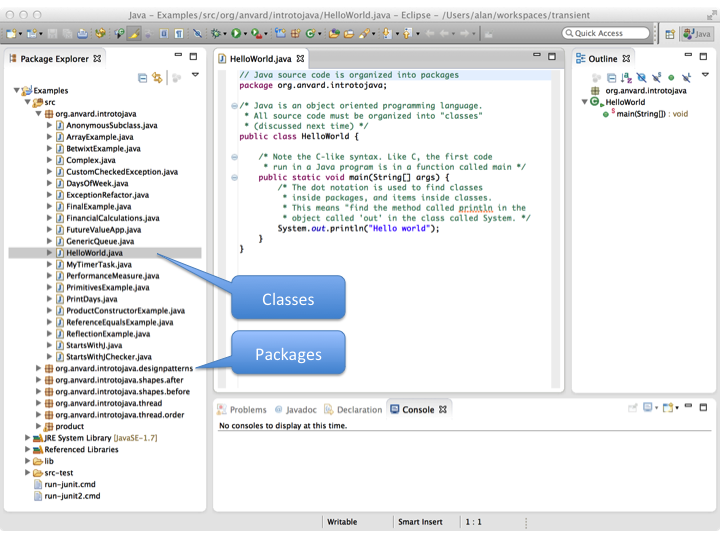
\includegraphics[width=0.9\textwidth]{screens/Slide1.png}}
\end{picture}
\end{frame}

\begin{frame}[fragile]
\frametitle{Running in Eclipse}
\begin{picture}(0,0)(-20,120)
     \put(0,0){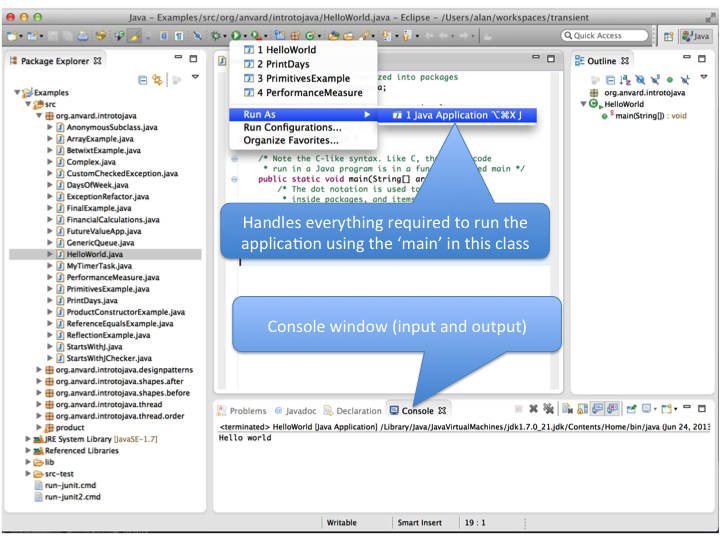
\includegraphics[width=0.9\textwidth]{screens/Slide2.png}}
\end{picture}
\end{frame}

\begin{frame}[fragile]
\frametitle{Debugging in Eclipse}
\begin{picture}(0,0)(-20,120)
     \put(0,0){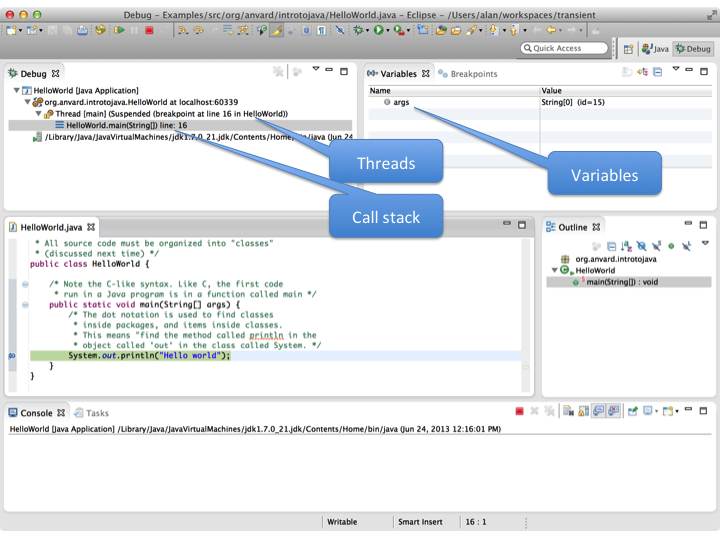
\includegraphics[width=0.9\textwidth]{screens/Slide3.png}}
\end{picture}
\end{frame}

\begin{frame}
\frametitle{Working in Eclipse}
\begin{itemize}
\item Eclipse performs continuous background compiling
\begin{itemize}
\item Errors are displayed immediately
\item The compiled class files are kept in an ``output'' folder (\texttt{bin} by default)
\end{itemize}
\item As dependencies are added to the ``build path'' for the project, they automatically become available for compiling and running
\item Eclipse can also connect to externally running Java programs (locally or on a network) for debugging
\end{itemize}
\end{frame}

\begin{frame}[fragile]
\frametitle{Compiling from the command line}
\begin{itemize}
\item The \texttt{javac} command is used for compiling from the command line
\begin{itemize}
\item For all but simple examples, it is not usually used directly
\item Later we will discuss build tools such as Apache Ant
\end{itemize}
\item Command line compiling must be done from the top level, not inside any packages
\item Any required libraries must be specified in the ``classpath''
\end{itemize}
This command creates a HelloWorld.class in the same directory as HelloWorld.java
\lstset{language=}
\begin{lstlisting}
$ javac org/anvard/introtojava/HelloWorld.java
\end{lstlisting}
\end{frame}

\begin{frame}[fragile]
\frametitle{Running from the command line}
\begin{itemize}
\item Java programs can be run directly using the command \texttt{java}
\item Later we will talk about packaging applications to avoid the command line
\item When running a Java program, we specify the ``main class'', so it is OK for multiple Java classes to have a ``main'' method
\end{itemize}
\lstset{language=}
\begin{lstlisting}
$ java -cp . org.anvard.introtojava.HelloWorld
Hello world
\end{lstlisting}
\lstset{language=}
\begin{lstlisting}
$ java -cp . org.anvard.introtojava.HelloName
What is your name? John Jacob Jingleheimer Schmidt
You have a long name.
Hello, John Jacob Jingleheimer Schmidt
\end{lstlisting}
\end{frame}

\begin{frame}[fragile]
\frametitle{The Java ``Classpath''}
\begin{itemize}
\item The classpath tells Java where to look for class files
\begin{itemize}
\item For compiling, this means already compiled code used as a dependency
\item For running, this means all classes the Java program will need
\end{itemize}
\item The ``classpath'' is just a list of locations to search for class files and other resources
\item The individual items can be directories, archive files, or arbitrary URLs
\item The standard Java library is always on the classpath
\item For our simple example, we just needed the current directory on the classpath
\end{itemize}
\lstset{language=}
\begin{lstlisting}
$ java -cp . org.anvard.introtojava.HelloWorld
Hello world
\end{lstlisting}
\end{frame}

\begin{frame}
\frametitle{Java Classpath issues}
\begin{itemize}
\item Classpath issues can be a source of frustration in running Java programs
\item Classes are found and loaded dynamically, so classpath issues might not be discovered until the program is running
\item Multiple classes on the classpath can have the same name
\begin{itemize}
\item The ``first'' one will be used
\item This can be confusing
\item Good package naming and organization will usually avoid this problem
\end{itemize}
\end{itemize}
\end{frame}

\begin{frame}
\frametitle{Next Time}
\begin{itemize}
\item Java Objects and Classes
\item Brief overview of Object-Oriented Programming
\item Distinction between primitive types and objects
\item Distinction between static and instance variables
\end{itemize}
\end{frame}

\begin{frame}
\frametitle{Credit in LMPeople}
\begin{center}
LMPeople Course Code: 071409ILT01
\end{center}
\end{frame}

\end{document}
